\section{Multilagen-PVD}
\label{multilayer}

Der PVD-Modus von Parsivald ist durch seine zyklische Arbeitsweise auch für Multilagensysteme geeignet, wie in diesem Abschnitt am Beispiel von Cu/Ni-Multilagen untersucht wird.

\subsection{Vorbetrachtung}
Die Wahl fiel auf Kupfer-Nickel-Systeme aufgrund der ähnlichen Atom- und Gittereigenschaften sowie die Verfügbarkeit eines kompatiblen \todo{cite lammps?}Potentiales.
Diese Systeme können per \todo{cite}Elektro\-deposition oder durch \todo{cite}Sputtern hergestellt werden, wobei üblicherweise Lagendicken von \todo{cite!}\SI{5}{\angstrom} bis \todo{cite! angstrom oder nm?}\SI{200}{\angstrom} produziert werden.
\todo{wirklich?}Durch Beschränkungen in der verfügbaren Rechenzeit beschränken sich die vorgestellten Simulationen auf Lagendicken unterhalb von \SI{10}{\angstrom}, allerdings sind größere Systeme technisch möglich.

An Multilagensystemen lassen sich strukturell neben den Dicken der einzelnen Lagen die Rauheiten aufeinanderfolgender Schichten besonders gut untersuchen.
Man betrachtet die Korrelation zwischen den einzelnen Schichten sowie den Verlauf der Rauheit bei späteren Schichten.
Für das Cu/Ni-System werden \todo{Aus welchem Hut wurde das gezaubert?}partiell korrelierte, kumulative Rauheiten erwartet, wobei Untersuchungen an den Gold- und Kupfer-Strukturen der letzten Kapitel eine systematische Überschätzung des Verlaufs der Rauheiten vermuten lassen\todo{Hut?}.

\subsection{Ergebnisse}

\begin{figure}[H]
  \captionsetup[subfigure]{singlelinecheck=false}
  \def\subfigwidth{7cm}
  \begin{subfigure}[t]{\subfigwidth}
    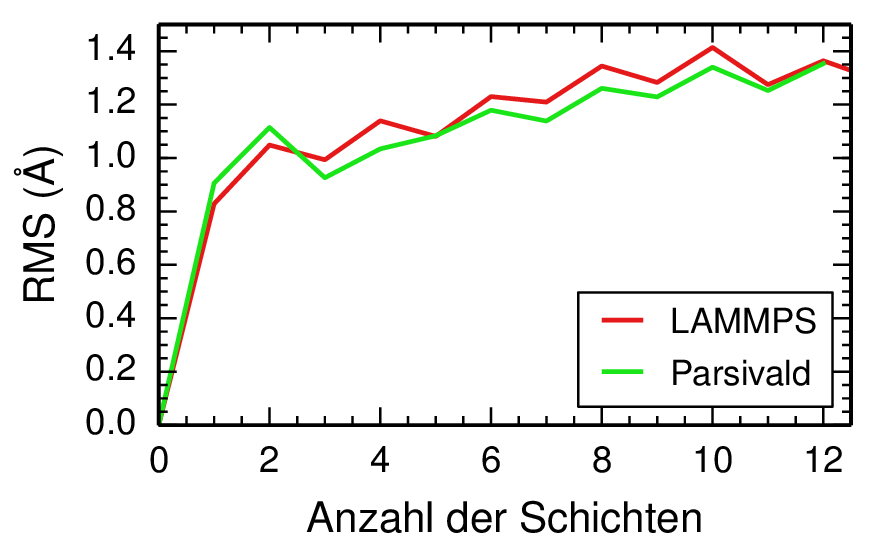
\includegraphics[width=\textwidth]{CuNi_layerroughness_comparison}
    \subcaption{
      Vergleich der Rauheit zwischen LAMMPS und Parsivald (Abb. \ref{fig:multilayerresults})
    }
  \end{subfigure}
  \hfill
  \begin{subfigure}[t]{\subfigwidth}
    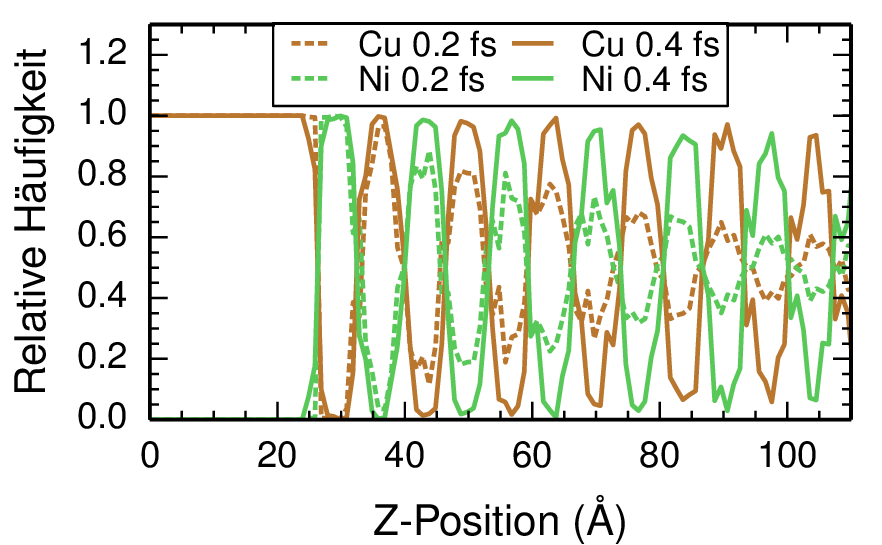
\includegraphics[width=\textwidth]{CuNi_atomdistribution_relax}
    \subcaption{Höhenverteilung der Kupfer- und Nickelatome innerhalb der Schicht}
  \end{subfigure}
  \caption[Ergebnisse der Multilagen-Abscheidung von Kupfer und Nickel]{
    Ergebnisse der Multilagen-Abscheidung von Kupfer und Nickel:
    Vergleich der zwischen LAMMPS und Parsivald (a) und Einfluss der Relaxationszeit auf die Schichtqualität in Parsivald (b)
  }
  \label{fig:multilayerplots}
\end{figure}

Die in Abbildung \ref{fig:multilayerresults} vorgestellten Ergebnisse zeigen erfolgreiches Multilagenwachstum per PVD-Modus mit Diffusion einzelner Atome in benachbarte Lagen.
Die Atome der verschiedenen Lagen setzen das fcc-Kristallgitter der vorherigen Lage fort, was durch die Ähnlichkeit der fcc-Gitterkonstanten zu erklären ist (\SI{3.52}{\angstrom} für Nickel, \SI{3.61}{\angstrom} für Kupfer, entspricht \SI{2.5}{\percent} Abweichung).
Bei größeren Systemen sind durch Verspannungen im Material Gitterversetzungen und -fehlstellen zu erwarten, die allerdings durch \todo{Wort}Finite-Size-Effekte unterdrückt sein können.

\begin{figure}[hp]
  \captionsetup[subfigure]{singlelinecheck=false}
  \def\subfigwidth{7cm}
  \begin{subfigure}[t]{\subfigwidth}
    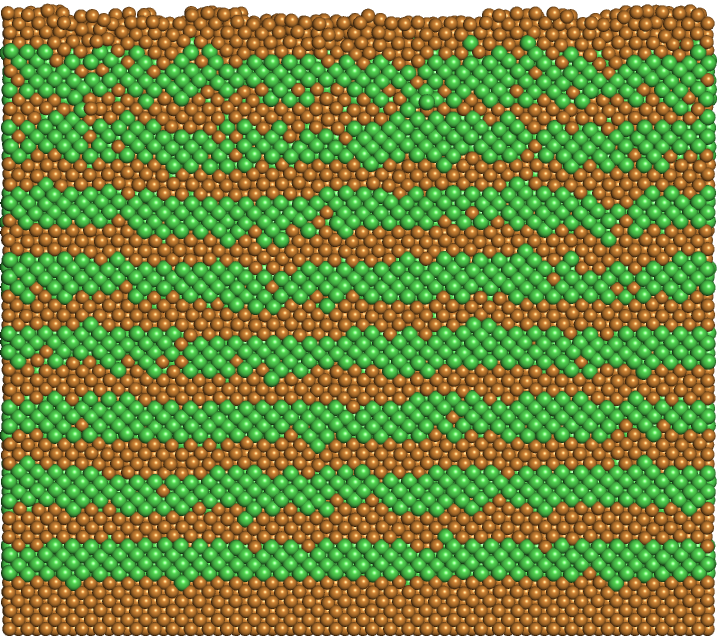
\includegraphics[width=\textwidth]{CuNi_profile_LAMMPS_nice}
    \subcaption{Profil einer per LAMMPS simulierten Multilagen-Abscheidung}
  \end{subfigure}
  \hfill
  \begin{subfigure}[t]{\subfigwidth}
    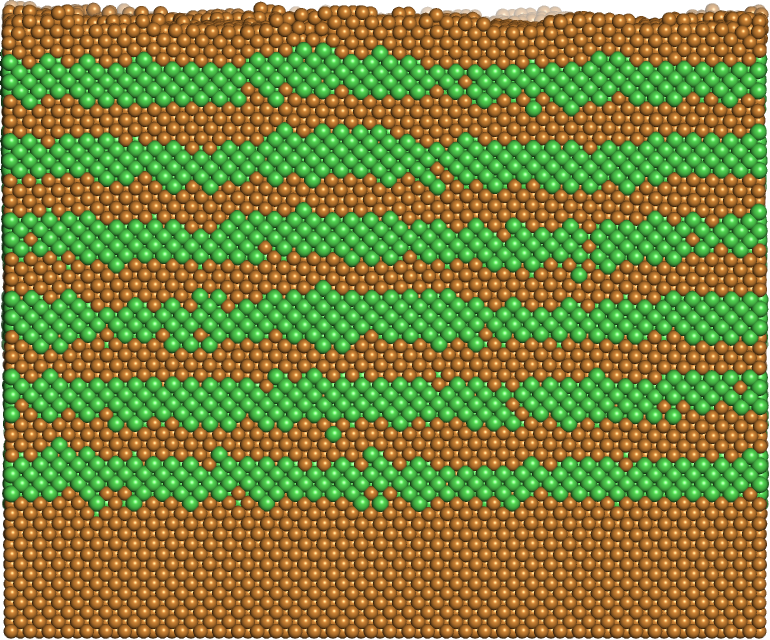
\includegraphics[width=\textwidth]{CuNi_profile_Parsivald}
    \subcaption{Profil einer per Parsivald simulierten Multilagen-Abscheidung}
  \end{subfigure}
  \caption[Vergleich zwischen Parsivald- und LAMMPS-Multilagenabscheidungen]{
    Vergleich zwischen Parsivald- und LAMMPS-Multilagenabscheidungen unter Nutzung optimierter Parameter.
  }
  \label{fig:multilayerresults}
\end{figure}

\begin{figure}[hp]
  \captionsetup[subfigure]{singlelinecheck=false}
  \begin{subfigure}[t]{8cm}
    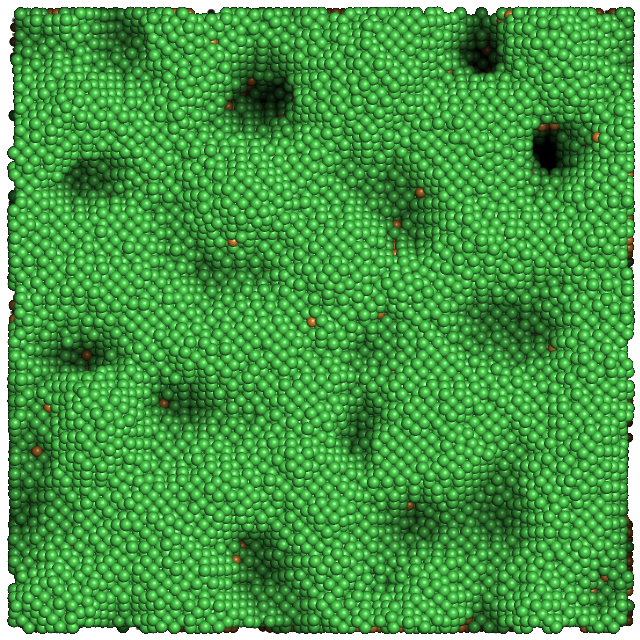
\includegraphics[width=\textwidth]{CuNi_surface8_noalpha}
    \subcaption{Draufsicht einer CuNi-Multi\-lagen\-ober\-fläche nach nur 4 Lagen (insgesamt \SI{60}{\angstrom})}
  \end{subfigure}
  \hfill
  \begin{subfigure}[t]{6cm}
    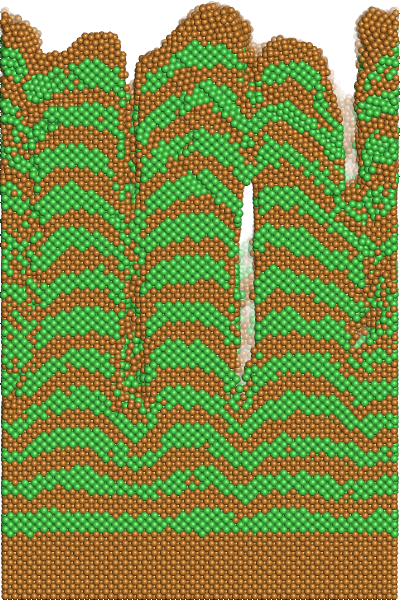
\includegraphics[width=\textwidth]{CuNi_columnfail}
    \subcaption{Dünnes Profil eines anderen Systemes nach 24 Lagen (\SI{180}{\angstrom})}
  \end{subfigure}
  \caption[Multilagen-Simulation mit willkürlichen Parametern]{
    Multilagen-Simulation mit Parsivald mit Parametern, die noch nicht auf genaue Darstellung des Systemes optimiert wurden.
    $t_\text{relax}$ liegt unterhalb der notwendigen Relaxationszeit.
  }
  \label{fig:multilayerfails}
\end{figure}
